\documentclass[11pt]{report}
\usepackage{graphicx} % Required for inserting images
\usepackage{titling}
\usepackage{geometry}
\usepackage{ulem}
\usepackage{titlesec}
\usepackage{titletoc}
\usepackage[style=numeric, sorting=none]{biblatex} % Styl numeryczny
\addbibresource{bibliografia.bib}
\usepackage[polish]{babel}
\AddToHook{cmd/section/before}{\clearpage}
\usepackage{longtable}
\usepackage{array}
\usepackage{listings}


% Styl rozdziału
\titleformat{\chapter}[block]
  {\normalfont\huge\bfseries} % Duża czcionka dla tytułu
  {\thechapter.} % Formatowanie numeru rozdziału
  {20pt} % Odstęp między numerem a tytułem
  {}

% Dodatkowe modyfikacje odstępów po tytule
\titlespacing*{\chapter}{0pt}{-20pt}{40pt}

% Ustawienia marginesów
\newgeometry{a4paper, tmargin=2.5cm, bmargin=2.5cm, lmargin=2.5cm, rmargin=2.5cm}

% Zwiększenie odstępów między liniami
\linespread{1.3}

\begin{document}

% Logo oraz nagłówek strony tytułowej
\posttitle{\\
\includegraphics[width=7cm]{LogoPolitechnikaMorskaWIiT.png}}

% Tytuł pracy
\title{\textbf{POLITECHNIKA MORSKA W SZCZECINIE\\
WYDZIAŁ INFORMATYKI I TELEKOMUNIKACJI}}
\author{\Large{Daniel Kropopek \\[1cm] 
\textbf{Projekt oraz wykonanie komputera 8-bitowego opartego o procesor MOS 6502} \\[0.5cm]
\textit{Design and creation of an 8-bit computer based on the MOS 6502 processor}}}

% Data
\date{Szczecin 2024}

% Tworzenie strony tytułowej
\maketitle

% Wstawianie plików i sekcji
\include{Oświadczenie}

% Spis treści
\tableofcontents

% Kolejne sekcje
\include{Wstęp}
\begingroup
\let\clearpage\relax
\begingroup
\let\clearpage\relax
\chapter{Projekt komputera 8-bitowego - zarys problematyki}
\section{Historia rozwoju komputerów osobistych}

W latach 80' ubiegłego wieku, nastąpił znaczny wzrost ilości osób posiadających komputer osobisty. 'Apple I', jeden z pierwszych komputerów osobistych, stworzony przez Steve'a Wozniaka w 1976 roku, był przeznaczony głównie dla tak zwanych hobbystów, ze względu na potrzebę samodzielnego montażu jego komponentów. Jego rewolucyjność polegała na nowatorskim podejściu do kontaktu z użytkownikiem, jako jeden z pierwszych komputerów wykorzystywał klawiaturę oraz monitor jako urządzenia peryferyjne, co pozwoliło na znacznie wygodniejszą obsługę.  Jego sukces zapoczątkował rozwój komputerów osobistych, które zaczęły pojawiać się na rynku w coraz większej liczbie.
\begin{figure}[h]
    \centering
    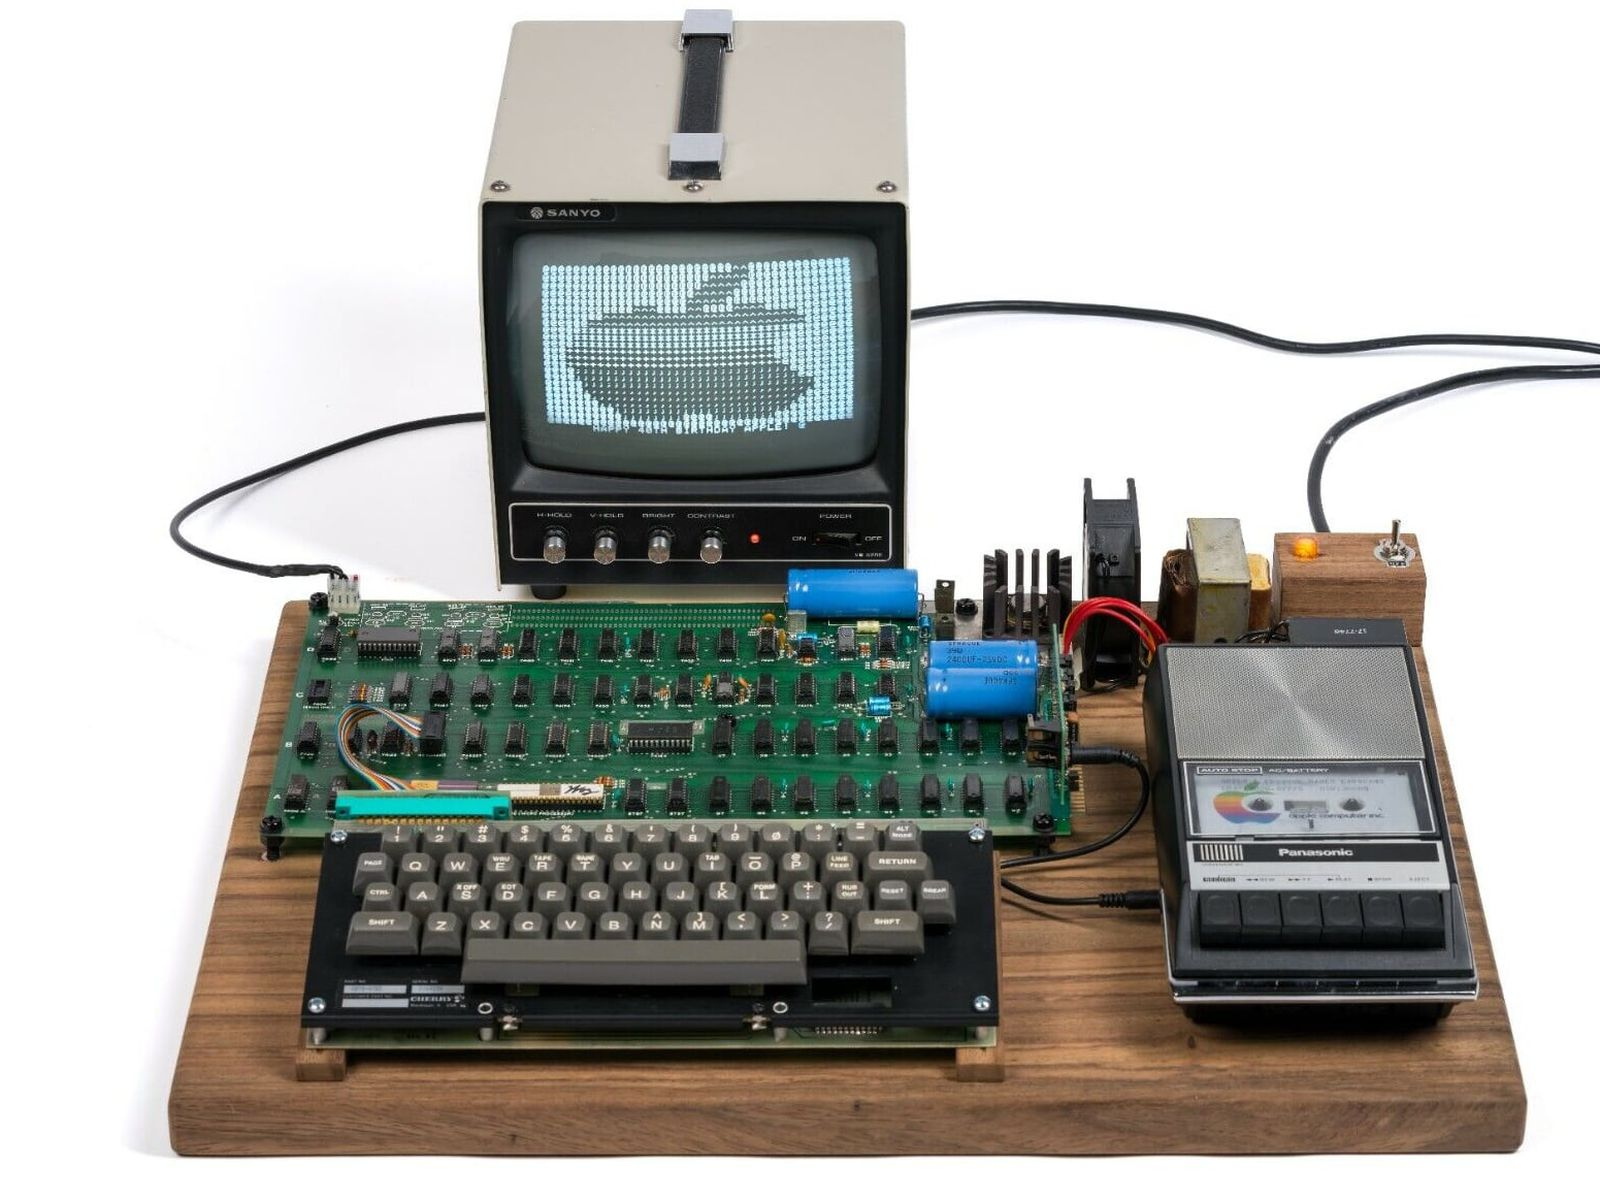
\includegraphics[width=0.8\textwidth]{images/apple-1.jpg} % Wstaw nazwę pliku z obrazem
    \caption{ \textit{Apple-1}}
    \label{fig:apple1} 
    \vspace{0.5em} % Odstęp między podpisem a źródłem
    \footnotesize Źródło: \parencite{macrumors2016}
\end{figure}
Czy 'Apple II', który umożliwia wyświetlanie kolorowego obrazu na monitorze, umożliwi odtwarzanie dźwięku, czy nawet pozwoli na użycie kart rozszerzeń. Na rynku pojawił się także komputer 'BBC Micro', stworzony we współpracy z brytyjską stacją BBC, którego głównym celem była edukacja i nauka programowania. Dzięki powyższym modelom komputerów osobistych stawały się one coraz bardziej przystępne cenowo i dostępne dla szerokiego grona użytkowników.
Wszystkie te komputery łączyła jedna cecha wspólna – procesor MOS 6502, który znacznie obniżał koszty produkcji. Dzięki temu urządzenia takie jak „Apple I”, „Commodore 64”, „BBC Micro” itp. były dostępne w znacznie niższych cenach, co czyniło je popularnymi nie tylko wśród entuzjastów technologii, ale także w codziennym użytkowaniu. Dostępność ta przyczyniła się do szybkiego wzrostu liczby użytkowników komputerów i stanowiła ważny krok w rozwoju technologii komputerowej.

\null\newpage
\section{Wybór procesora MOS 6502 jako kluczowego elementu projektu.}

Początki komputerów osobistych zdominowały głównie dwa procesory, MOS 6502 oraz procesor Zilog Z80. Procesor firmy MOS, teraz wykupionej przez firmę Western Design Center, jest dalej produkowany oraz dostępny w sprzedaży. Firma Zilog wycofała się z produkcji procesora Z80 na początku 2024 roku \parencite{ithardware2024}. 

\begin{figure}[h]
    \centering
    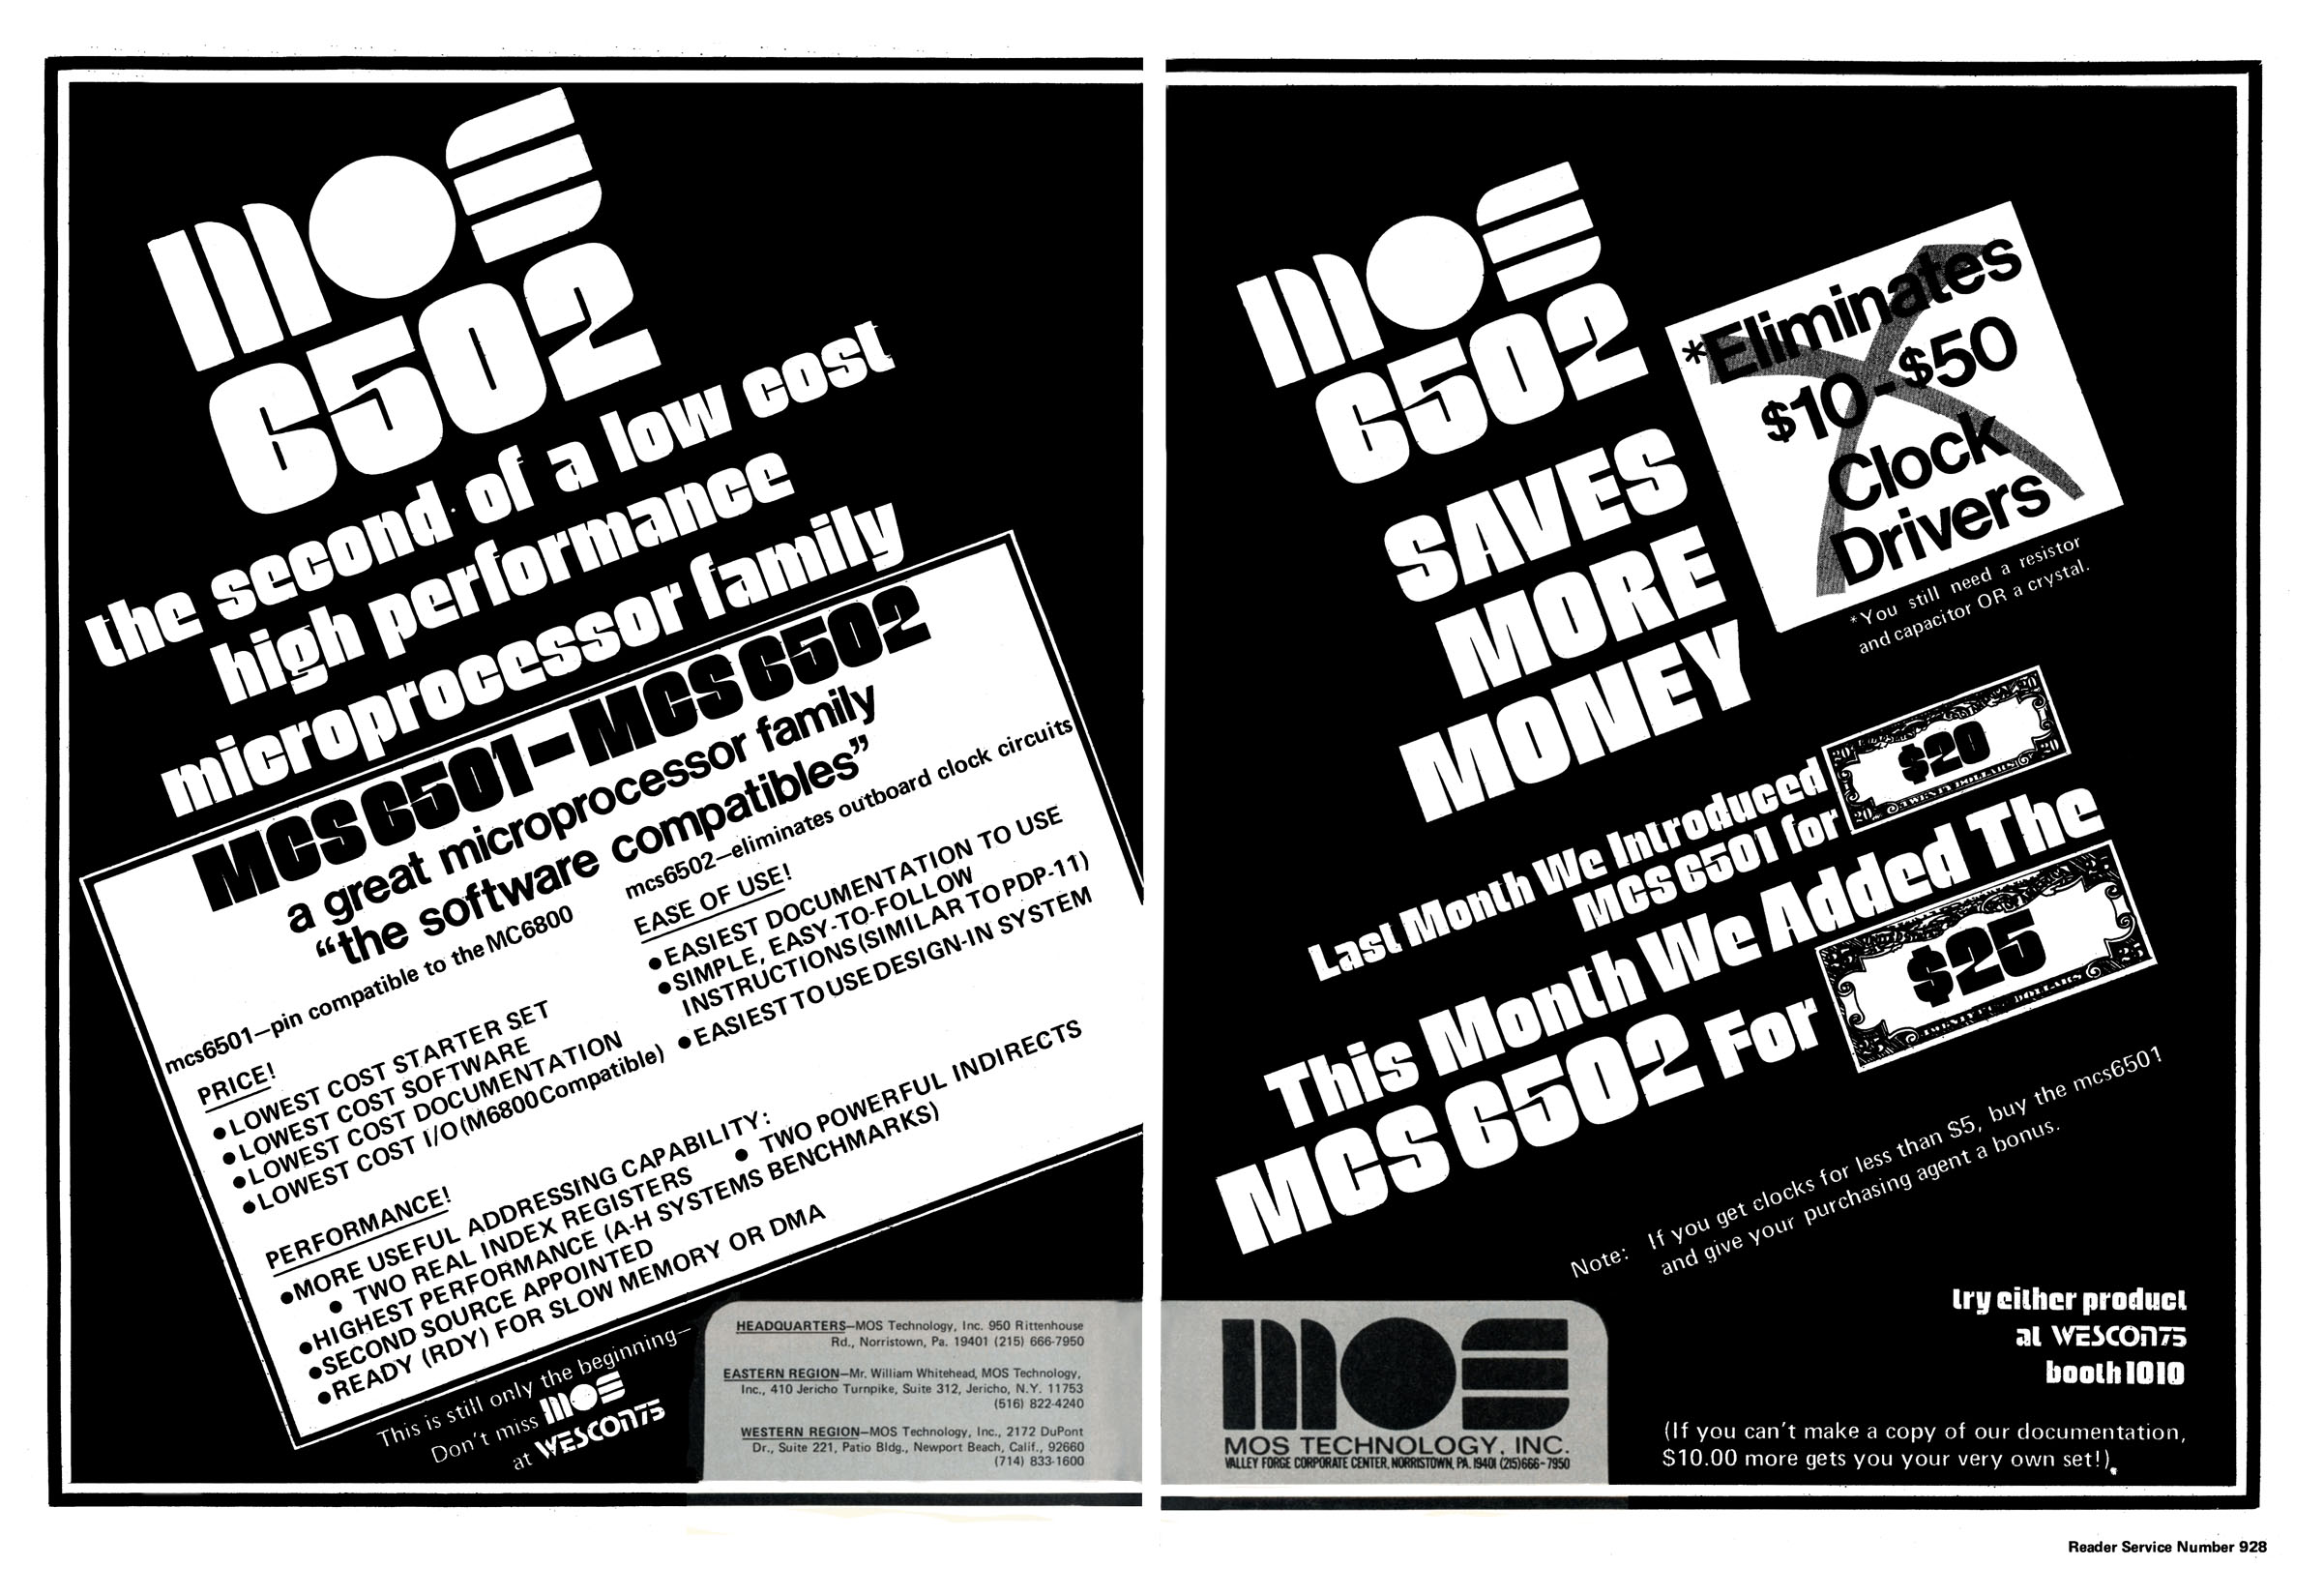
\includegraphics[width=0.8\textwidth]{images/MOS_6501_6502_Ad_Sept_1975.jpg} % Wstaw nazwę pliku z obrazem
    \caption{ \textit{Reklama procesora mos 6502 z 1975 roku}}
    \label{fig:apple1} 
    \vspace{0.5em} % Odstęp między podpisem a źródłem
    \footnotesize Źródło: \parencite{wikipedia6502}
\end{figure}

Procesor 8-bitowy posiada o wiele łatwiejszą architekturę do zrozumienia niż procesor 16-bitowy lub procesor o jeszcze większej magistrali. Rozwiązanie takie umożliwi łatwiejszą pracę nad komputerem. Dzisiaj dalej popularne są mikroprocesory wykorzystujące 8-bitową magistralę, takie jak poprzednio pisane Z80 oraz 65C02 (wersja CMOS układu 6502) oraz chociażby popularny układ ATmega328P w architekturze ARM wykorzystywany w Arduino. Procesor ARM został zaprojektowany przez Sophie Wilson, która także pomagała w tworzeniu BBC Micro. Procesory architektury ARM mają podobny rejestr stanu do procesora 6502. Jednak jest to nie jedyny dowód na podobieństwa tych dwóch procesorów. Inżynierowie firmy Acorn, podczas tworzenia zbioru instrukcji dla procesora ARM\parencite{statusregisterARm}, inspirowali się krótkimi i prostymi instrukcjami w procesorze 6502, które były zbliżone do procesorów architektury RISC \parencite{atack1993}.

\null\newpage
\section{Cele projektu}
Celem niniejszej pracy inżynierskiej jest stworzenie komputera, który umożliwi naukę programowania niskopoziomowego oraz pracy z mikrokontrolerami z rodziny AtMega.

\endgroup
\endgroup
\begingroup
\let\clearpage\relax
\chapter{Projekt komputera 8-bitowego}
\section{Analiza układów wchodzących w skład komputera}
\subsection{Procesor MOS 6502}
Architektura procesora MOS 6502 oparta jest na architekturze von Neumanna, jest to rodzaj architektury, w którym dane programu, są przechowywane w tym samym miejscu co kod programu. Oznacza to, że w pamięci RAM możemy mieć zapisane czyste dane, na przykład zapisane adresy w stosie, a w kolejnych adresach kod programu który właśnie wykonujemy. Wewnętrzna struktura procesora jest zaprojektowana w sposób umożliwiający zrównoważoną wydajność pomimo posiadania tylko dwóch rejestrów, oraz co najważniejsze, jej budowa jest prosta, co zostało osiągnięte przez użycie zmniejszonej ilości tranzystorów w porównaniu do innych procesorów z tego okresu.
Główne komponenty procesora to między innymi:
\begin{itemize}
\item Rejestry
\item Jednostka arytmetyczno-logiczna
\item Jednostka zegara i pomiaru czasu
\item jednostka sterująca 
\end{itemize}
\hfill \break
\textbf{Rejestry} wewnętrzne rejestry, a więc komórki pamięci umieszczone wewnątrz procesora o rozmiarach 8 oraz 16 bitów zależnie od roli, jaką pełnią, służą do przechowywania  tymczasowych obliczeń, adresów pamięci oraz funkcji indeksowania. Procesor zawiara rejestry przedstawione w tabeli.

\begin{longtable}{|p{5cm}|p{11cm}|}
\hline
\textbf{Rejestr} & \textbf{Opis} \\ \hline
\endfirsthead
\hline
\textbf{Rejestr} & \textbf{Opis} \\ \hline
\endhead
\hline
\endfoot
\hline
\caption{Rejestry procesora i ich funkcje} \\
\endlastfoot

Akumulator (A) & Główny rejestr dla wykonywanych operacji arytmetycznych i logicznych. Jest bezpośrednio połączony z jednostką arytmetyczno-logiczną. \\ \hline
Rejestry indeksów (X i Y) & Rejestry pomocnicze używane w trybach adresowania indeksowanego i jako liczniki w procesach iteracyjnych. \\ \hline
Licznik programu (PC) & Jest to 16-bitowy rejestr, którego zadaniem jest ustalenie adresu pamięci, w którym znajduje się następna instrukcja, która ma zostać wykonana. Jego wartość jest zwiększana automatycznie podczas cyklu pobierania lub zmieniana przez odpowiednie instrukcje (np. JMP, JSR). \\ \hline
Wskaźnik stosu (S) & 8-bitowy rejestr wskazujący na wierzch stosu, którego adres oznacza pierwszą stronę pamięci, od adresu \$0100 do \$01FF. Strony pamięci zostaną opisane w temacie pamięci RAM. \\ \hline
Rejestr stanu procesora (P) & 8-bitowy rejestr zawierający wartości zależne od wyniku ostatnio wykonanej operacji, nazywane flagami. Bity w tym rejestrze przyjmują format "NV1BDIZ", gdzie każdy z bitów odpowiada innej fladze. Flagi w procesorze 6502 to:

\begin{itemize}
\item \textbf{N Flaga ujemności}  
Flaga ta zostanie ustawiona po każdej operacji arytmetycznej (gdy do któregokolwiek z rejestrów A, X lub Y wpisywana jest wartość).

\item \textbf{V Flaga przeładowania}  
Podobnie jak flaga ujemności, flaga ta jest przeznaczona do użycia z 8-bitowymi liczbami całkowitymi ze znakiem. Na flagę będą miały wpływ dodawanie i odejmowanie, instrukcje PLP, CLV i BIT oraz sygnał sprzętowy SO. Sygnał SO (Set Overflow) jest dostępny w procesorze 6502 (choć nie był dostępny we wszystkich procesorach z rodziny 65XX) i służy do ustawienia flagi V. Umożliwia to reakcję na działanie I/O w czasie równym lub krótszym niż trzy cykle zegara, gdy używana jest instrukcja BVC rozgałęziająca się do samej siebie (\$50 \$FE). Instrukcja CLV czyści flagę V, a instrukcje PLP i BIT kopiują wartość flagi z bitu 6 najwyższego wpisu stosu lub z pamięci. Po dodaniu lub odjęciu binarnym flaga V zostanie ustawiona w przypadku przepełnienia znaku, w przeciwnym razie zostanie wyczyszczona. 

\item \textbf{1 Flaga nieużywana} 
Zgodnie z obecnym stanem wiedzy, flaga ta ma zawsze wartość 1.

\end{itemize} \\ \hline \\
Rejestr stanu procesora (P) &
\begin{itemize}
\item \textbf{B Flaga przerwań} 
Flaga ta służy do rozróżniania przerwań programowych (BRK) od przerwań sprzętowych (IRQ lub NMI). Flaga B jest zawsze ustawiona, z wyjątkiem sytuacji, gdy rejestr P jest wypychany na stos podczas skoku do programu obsługi przerwań w celu przetworzenia tylko przerwania sprzętowego. Oficjalna dokumentacja NMOS 65xx twierdzi, że instrukcja BRK może powodować tylko skok do wektora IRQ (\$FFFE). Jeśli jednak podczas wykonywania instrukcji BRK wystąpi przerwanie NMI, procesor wykona skok do wektora NMI (\$FFFA), a rejestr P zostanie wepchnięty na stos z ustawioną flagą B.

\item \textbf{D Flaga trybu dziesiętnego} 
Flaga ta służy do wyboru trybu dziesiętnego (kodowanego binarnie) dla dodawania i odejmowania. W większości aplikacji flaga ta ma wartość zero.

\item \textbf{I Flaga wyłączenia przerwań} 
Flaga ta służy do zapobiegania przeskakiwaniu procesora do wektora obsługi IRQ (\$FFFE), gdy linia sprzętowa -IRQ jest aktywna. Flaga zostanie automatycznie ustawiona po odebraniu przerwania, dzięki czemu procesor nie będzie przeskakiwał do procedury obsługi przerwań, jeśli sygnał -IRQ pozostanie niski przez kilka cykli zegara.

\item \textbf{Z Flaga Zerowa}
Flaga Zero zostanie zmieniona w tych samych przypadkach, co flaga ujemna. Ogólnie rzecz biorąc, zostanie ona ustawiona, jeśli rejestr arytmetyczny jest ładowany z wartością zero, a wyczyszczona w przeciwnym razie. 

\end{itemize} \\ \hline \\
Rejestr stanu procesora (P) &
\begin{itemize}

\item \textbf{C Flaga przenoszenia}
Flaga ta jest używana w dodawaniu, odejmowaniu, porównywaniu i rotacji bitów. W dodawaniu i odejmowaniu działa jako 9 bit i pozwala na łączenie operacji w celu obliczenia liczb większych niż 8-bitowe. Podczas odejmowania flaga Carry jest ujemna w stosunku do Borrow: jeśli wystąpi przepełnienie, flaga zostanie wyczyszczona, w przeciwnym razie ustawiona. Porównania są szczególnym przypadkiem odejmowania: zakładają, że flaga Carry jest ustawiona, a flaga Decimal jest wyczyszczona i nie przechowują nigdzie wyniku odejmowania. Wszystkie z nich przechowują bit, który jest obracany do flagi przenoszenia. Instrukcje przesunięcia w lewo to ROL i ASL. ROL kopiuje początkową flagę Carry do najniższego bitu bajtu; ASL zawsze ją czyści. Podobnie, instrukcje ROR i LSR przesuwają w prawo.

\end{itemize} \\ \hline

\end{longtable}


Procesor 6502 zawiera kilka wewnętrznych rejestrów niezbędnych do wykonywania instrukcji i zarządzania danymi. Accumulator (A) jest głównym rejestrem używanym do operacji arytmetycznych i logicznych, współpracującym bezpośrednio z ALU. Rejestry indeksowe (X i Y) pomagają w adresowaniu indeksowym i działają jako liczniki podczas procesów iteracyjnych. Licznik programu (PC) to 16-bitowy rejestr, który śledzi adres pamięci następnej instrukcji do wykonania, automatycznie zwiększany podczas cyklu pobierania lub wyraźnie modyfikowany przez instrukcje sterujące, takie jak JMP. Wskaźnik stosu (SP) to 8-bitowy rejestr wskazujący na szczyt stosu, który znajduje się na stronie pamięci \$01 i ma kluczowe znaczenie dla obsługi wywołań podprogramów, przerwań i tymczasowego przechowywania danych. Wreszcie, Processor Status Register (P) to 8-bitowy rejestr, który przechowuje flagi odzwierciedlające wyniki operacji, w tym flagę Carry (C) dla przeniesień arytmetycznych lub operacji pożyczania, flagę Zero (Z) dla wyników równych zero, flagę Negative (N) odzwierciedlającą MSB w celu wskazania wartości ujemnych oraz flagę Overflow (V) sygnalizującą przepełnienie arytmetyczne ze znakiem.

Graficzne przedstawienie zależności między rejestrami, oraz polecenia służące do zmiany wartości w danym rejestrze prezentują się następująco:
\begin{figure}[h]
    \centering
    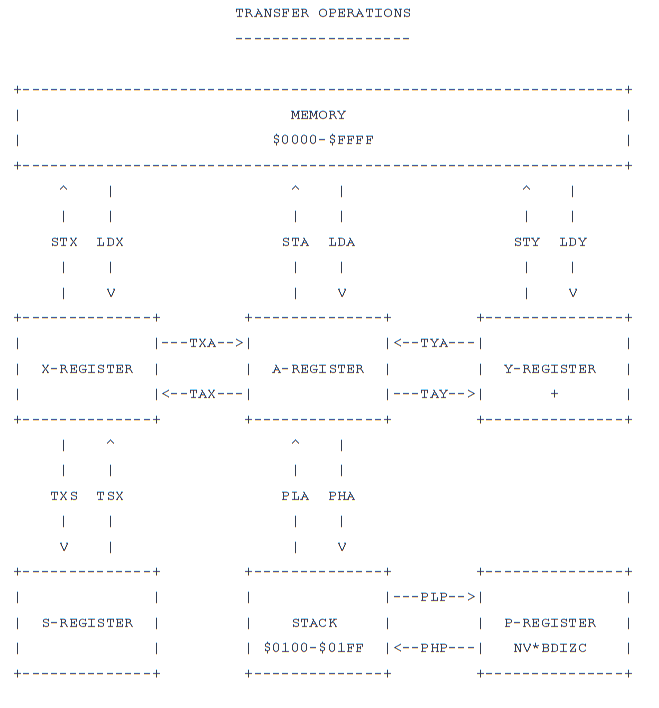
\includegraphics[width=0.8\textwidth]{images/Transfer_Operations.png} % Wstaw nazwę pliku z obrazem
    \caption{ \textit{Rejestry procesora MOS 6502}}
    \label{fig:Transfer_Opertaions} 
    \vspace{0.5em} % Odstęp między podpisem a źródłem
    \footnotesize Źródło: Opracowanie własne na podstawie \parencite{sander_cederlof_6502}
\end{figure}

\endgroup

\listoftables
\printbibliography

\end{document}
